\begin{figure}
  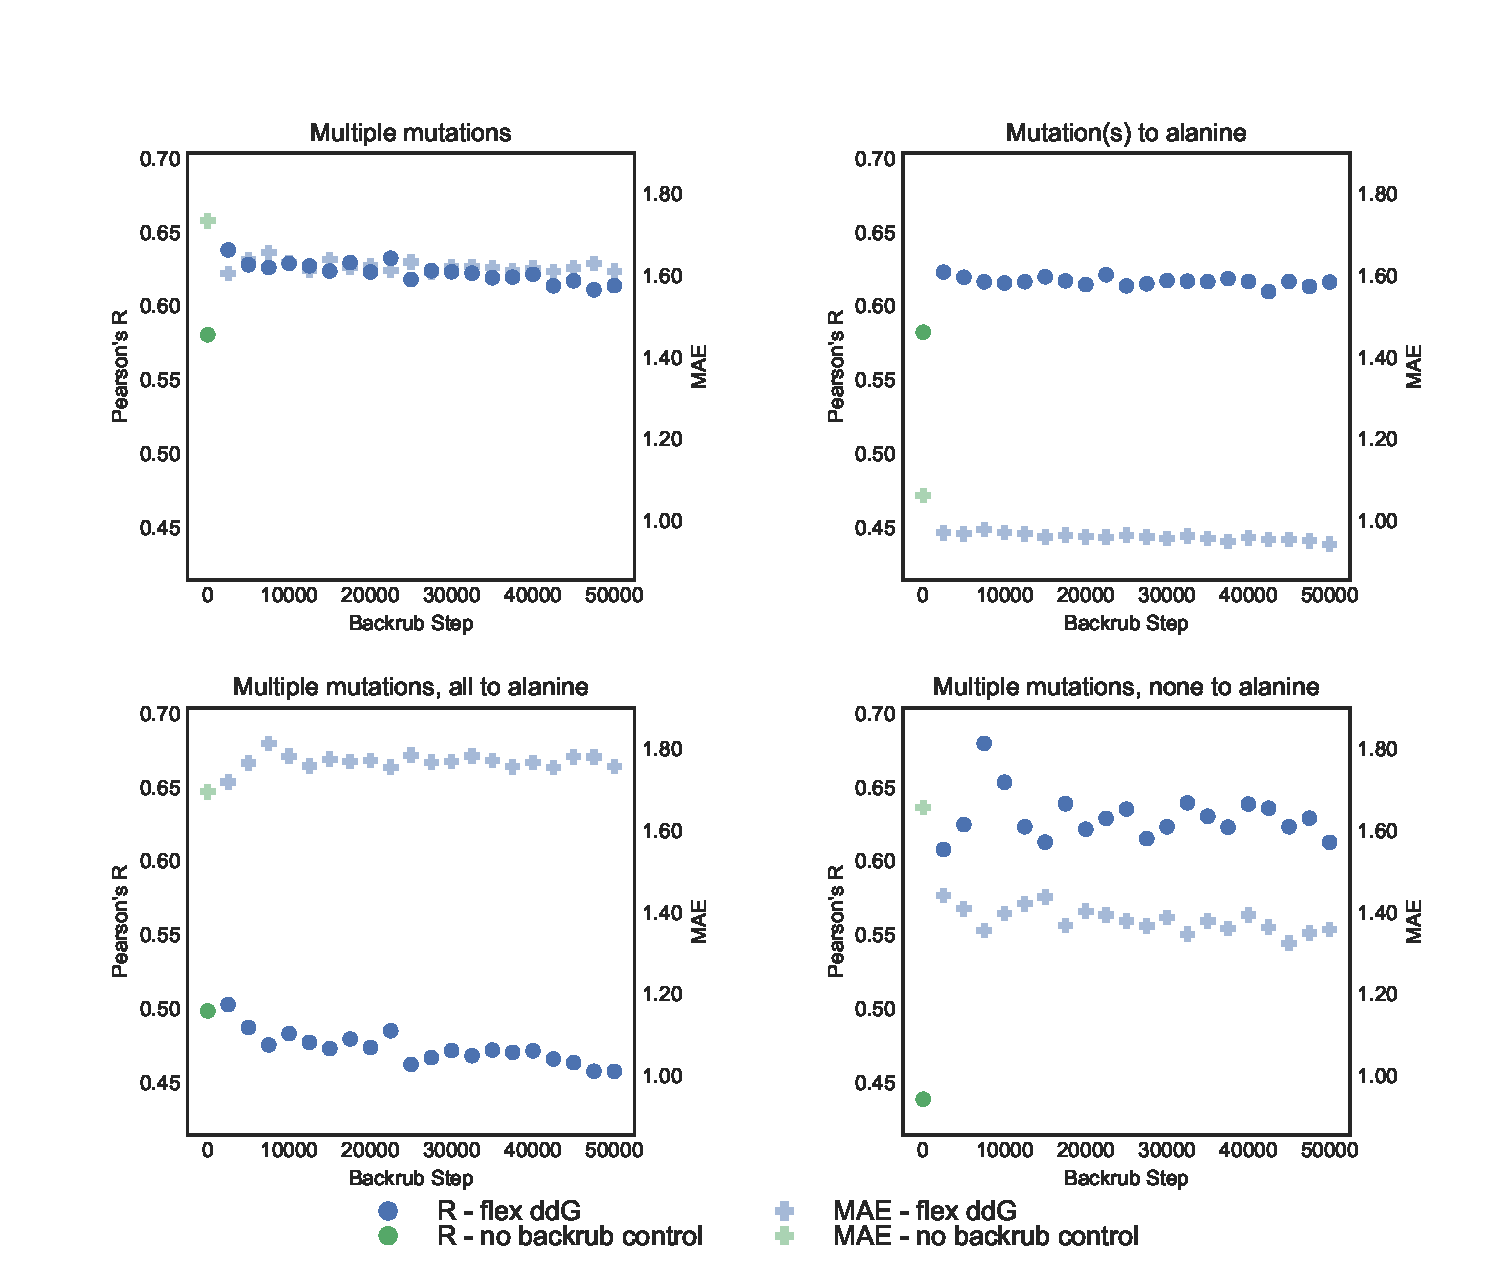
\includegraphics[width=\textwidth,keepaspectratio]{steps-v-corr_mult.pdf}
  \caption[Flex ddG performance vs. number of backrub steps]{
    Correlation (Pearson's R) and MAE (Mean Absolute Error) vs. number of backrub steps, on the complete ZEMu set, and subsets.
    Pearson's R is shown as circles, and MAE as faded plusses.
Predictions generated with the Flex ddG protocol are shown in blue.
Predictions generated with the no backrub control protocol are shown in green.
    A selection of key data underlying this figure can be found in \cref{tab:steps-v-corr_mult-underlying-data}.
    (a) (a) - Multiple mutations (n=273)
    (b) (b) - Mutation(s) to alanine (n=939)
    (c) (c) - Multiple mutations, all to alanine (n=191)
    (d) (d) - Multiple mutations, none to alanine (n=45)
  } \label{fig:steps-v-corr_mult}
\end{figure}
